\graphicspath{{chapters/images/ltee/}}
\chapter{LTEE}

\section{Long-term evolution experiment}
\subsection{Historical contingency and the evolution of a key innovation in an experimental population of E.coli}
Some notes on evolution:  Stephen Jay Gould maintained that historical contingencies make evolution largely unpredictable. Although each change on an evolutionary path has some causal relation to the circumstances in which it arose, outcomes must eventually depend on the details of long chains of antecedent states, small changes in which may have enormous long-term repercussions.  
'Evolutionary preadaptation’  entails that the right context is needed to develop and survive.
The outcome of evolution is largely unpredictable. 
The aim of the paper is to study evolution over time.  Selective pressure,  is not applied, scientists just propagate E. coli strains and try to understand what happens qualitatively over time.
\\
\\
\noindent
To address the repeatability of evolutionary trajectories and outcomes, the long-term evolution experiment (LTEE) with Escherichia coli was started in 1988 with the founding of 12 populations from the same clone. These populations were initially identical except for a neutral marker (not on a gene) that distinguished six lines from six others. They have since been propagated by daily 1:100 serial transfer in DM25, a minimal medium containing 25 mg/liter glucose as the limiting resource. Environmental conditions have been controlled, constant, and identical for all 12 lines. To date, each population has evolved for 44,000 generations, and samples have been frozen every 500 generations, providing a rich ‘‘fossil record’’. The founding strain is strictly asexual, and thus populations have evolved by natural selection and genetic drift acting on variation generated solely by spontaneous mutations that occurred during the experiment. Thus, the LTEE allows the examination of the effects of contingency that are inherent to the core evolutionary processes of mutation, selection, and drift. Random mutations will probably lead to a neutral change, negative mutations to disruption and beneficial mutations to adaptive evolution. Genetic drift is the change in the frequency of an existing gene variant (allele) in a population due to random sampling of organisms.
\\
\\
\noindent
Parallels: previous analyses of this experiment have shown numerous examples of parallel phenotypic and genetic evolution. 
\begin{itemize}
\item All twelve populations underwent rapid improvement in fitness that decelerated over time. 
\item All evolved higher maximum growth rates on glucose (only food source), shorter lag phases upon transfer into fresh medium, reduced peak population densities, and larger average cell sizes relative to their ancestor. 
\item Ten populations evolved increased DNA supercoiling, and those populations examined to date show parallel changes in global gene-expression profiles. 
\item At least three genes have substitutions in all 12 populations , and several others have substitutions in many populations, even though most loci harbor no substitutions in any of them. 
\end{itemize}
\noindent
Divergence
\begin{itemize}
\item Four populations have evolved defects in DNA repair, causing mutator phenotypes. 
\item There is subtle, but significant, between population variation in mean fitness in the glucose-limited medium in which they evolved. 
\item In media containing other carbon sources, such as maltose or lactose, the variation in performance is much greater. And while the same genes often harbor substitutions, the precise location and details of the mutations almost always differ between the populations. 
\end{itemize}

\noindent
The process of evolution is a combination of spontaneous mutations and fluctuations of frequency when we keep the environment constant without selecting. Just because we have a genetic change, it does not mean that something relevant is occurring in the population. If turbidity is present in a flask, it means that the bacterial content is higher; in order to check what’s going on we can employ optical density analysis.
\\
\\
\noindent
DM25 medium contains not only glucose, but also citrate at a high concentration (to control pH differences). The inability to use citrate as an energy source under oxic conditions has long been a defining characteristic of E. coli as a species. The only known barrier to aerobic growth on citrate is its inability to transport citrate under oxic conditions - E.coli has a complete tricarboxylic acid cycle, and can thus metabolize citrate internally during aerobic growth on other substrates the genes are present, but there is no transport.
\\
\\
\noindent
Atypical (mutated) E. coli can grow aerobically on citrate (Cit+). They have been isolated from agricultural and clinical settings, and were found to harbor plasmids, presumably acquired from other species, that encode citrate transporters. None of the 12 LTEE populations evolved the capacity to use the citrate that was present in their environment for over 30,000 generations. During that time, each population experienced billions of mutations, far more than the number of possible point mutations in the 4.6- million-bp genome. This ratio implies, to a first approximation, that each population tried every typical one-step mutation many times. 
The Cit variant arose within the LTEE and is not a contaminant. 

\subsection{Genomic analysis of a key innovation in an experimental E. coli population}
At least three distinct clades coexisted for more than 10,000 generations before its emergence. The Cit+ trait originated in one clade by a tandem duplication that captured an aerobically expressed promoter for the expression of a previously silent citrate transporter. The clades varied in their propensity to evolve this novel trait, although genotypes able to do so existed in all three clades, implying that multiple potentiating mutations arose during the population’s history. Findings illustrate the importance of promoter capture and altered gene regulation in mediating the exaptation events that often underlie evolutionary innovations. 
\\
\\
\noindent
The Cit+ trait was actualized by a duplication mutation that created a new regulatory module by placing a copy of the citT gene that encodes a citrate-succinate antiporter under the control of a promoter (mk) that supports expression under aerobic conditions. This mutation results in the CitT transporter being expressed when oxygen is present, permitting growth on citrate. 
After Cit+ evolved more mutations occurred, the turning point led to many modifications. Since the ancestral strains are conserved, it was possible to go back in time, they start propagating and witnessed the same outcome over and over again. Keep in mind that it does not always occur in the same way, there are some differences in the tandem duplication position (the exact position is chosen at random, the gene is the same). It should be stochastic, but it seems to be quite deterministic. In these experiments, they observed 19 new, independent instances of Cit+ re-evolution, but only when starting from clones isolated from after generation 20,000. 
Some of the mutations are in the control regions, other in the gene itself. Note that the frequency of gltA1 almost got lost, but then was fixed. This specific mutation is particularly relevant for Cit+; it has to do with the interaction between citrate synthetase and NADH interaction. 

\begin{figure}[h]
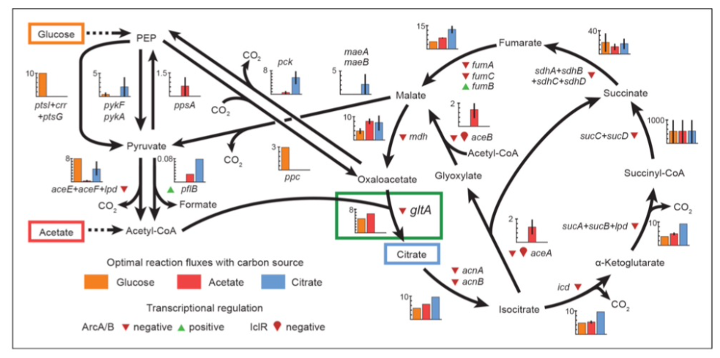
\includegraphics[width=1\textwidth, center]{flux_balance_analysis}
\caption{\label{fig:flux_an} Flux balance analysis}
\end{figure}

\noindent
Here we have 3 possible carbon sources: glucose, acetate and citrate. Acetate is not present in the medium, it is a waste product from some E. coli metabolism; it can be eaten in certain conditions.
The aim of E. coli is to optimize the rate of biomass accumulation when utilizing a single carbon source: either glucose, acetate, or citrate. E. coli excretes acetate as an overflow metabolite during growth on glucose and then switches to utilizing this acetate after glucose is depleted. Both the evolved iclR and arcB alleles are loss-of-function mutations that derepress expression of enzymes needed for acetate assimilation. The results of the FBA modeling agree with experimental observations: the combined effects of derepressing the IclR and ArcAB regulons via the iclR and arcB mutations and alleviating NADH-mediated allosteric inhibition of CS via the gltA1 mutation are beneficial for growth on acetate because they increase flux values for these reactions toward levels that are optimal for this substrate. 
\\
\\
\noindent
This metabolic program is thought to potentiate the evolution of Cit+ by increasing the production of C4-dicarboxylates (succinate, fumarate, and malate) which can be exported in exchange for citrate uptake by the CitT antiporter. Under Cit++ conditions in which citrate is the primary carbon source, FBA predicts that drastically reducing flux through the CS reaction is required to achieve an optimal growth rate which also agrees with our finding that beneficial gltA2 mutations that decrease CS activity evolved at this point in the LTEE. 
\\
\\
\noindent
The overall process can be summarized as following: E. coli eats all the glucose, then eats acetate to produce succinate, fumarate, etc.  and finally eats citrate and transport it through the CitT antiporter. Thanks to citrate it is also possible to produce glucose through gluconeogenesis.
\\
\\
\noindent
The first gltA mutation is advantageous when no citrate is utilized but deleterious when citrate is metabolized. The opposite is seen with the additional gltA mutations. Without gltA mutation, it will not be possible to survive on citrate. Epistatic interactions between gltA1 and the citT mutation in this evolved genetic background prevented a massive fitness defect that would have almost certainly led to the rapid extinction of any newly evolved Cit+ cells before this rudimentary trait could be refined to the advantageous Cit+ + phenotype by further mutations. The order of mutation matters! 
Lenski and his colleagues concluded that the evolution of the Cit+ function in this one population arose due to one or more earlier, possibly nonadaptive, "potentiating" mutations that increased the rate of mutation to an accessible level. The data suggested that citrate usage involved at least two mutations subsequent to these "potentiating" mutations. 
This LTEE population can be thought of as having evolved through three metabolic epochs: 
\begin{enumerate}
\item glucose utilization was optimized, leading to greater acetate accumulation; 
\item acetate utilization was optimized in conjunction with further improvements in glucose growth; 
\item citrate utilization was discovered and optimized. 
\end{enumerate}

Blount et al. suggested that this pattern might be typical of how novel traits in general evolve, and proposed a three-step model of evolutionary innovation: 
\begin{itemize}
\item Potentiation: a genetic background evolves in which a trait is mutationally accessible, making the trait's evolution possible (adjacent possible, Stuart Kauffman)
\item Actualization: a mutation occurs that produces the trait, making it manifest, albeit likely in a weak form. 
\item Refinement: Once the trait exists, if it provides selective benefit, mutations will accumulate that improve the trait, making it effective. This phase is open-ended, and will continue so long as refining mutations arise and the trait remains beneficial 
\end{itemize}
